% !TeX root = ../correctness-deciders.tex

\newpage
\section{Cyclers}\label{sec:cyclers}

\begin{figure}[h!]
  \centering
  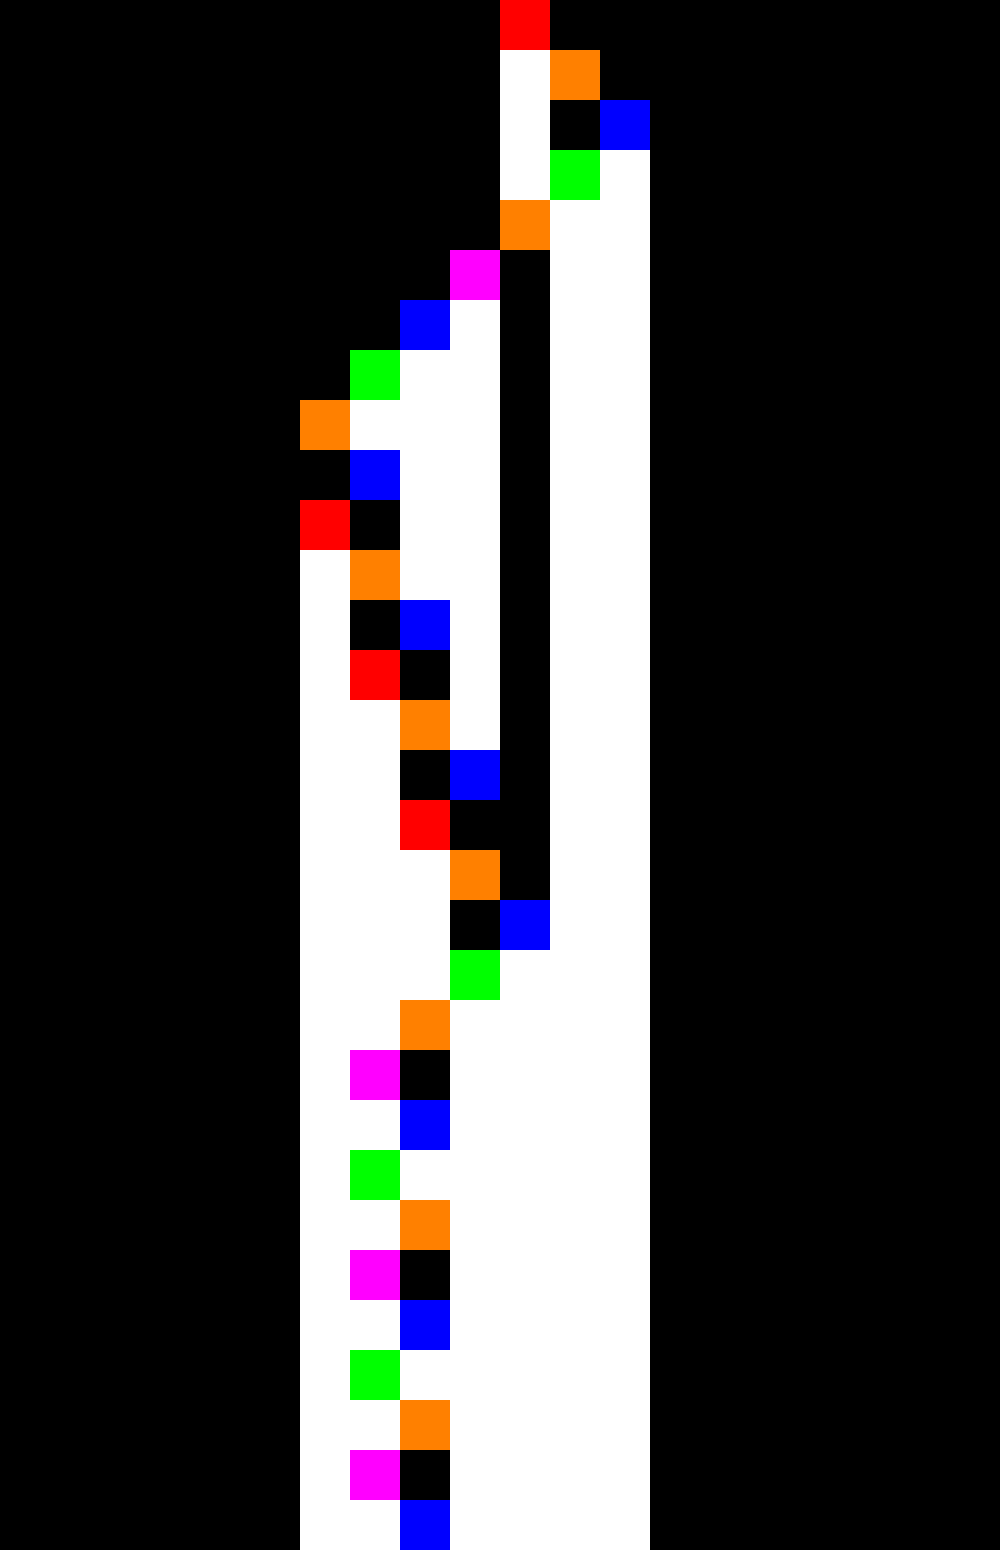
\includegraphics[width=0.4\textwidth]{figures/space-time-diagrams/cycler_279081.pdf}
  \hspace{2ex}
  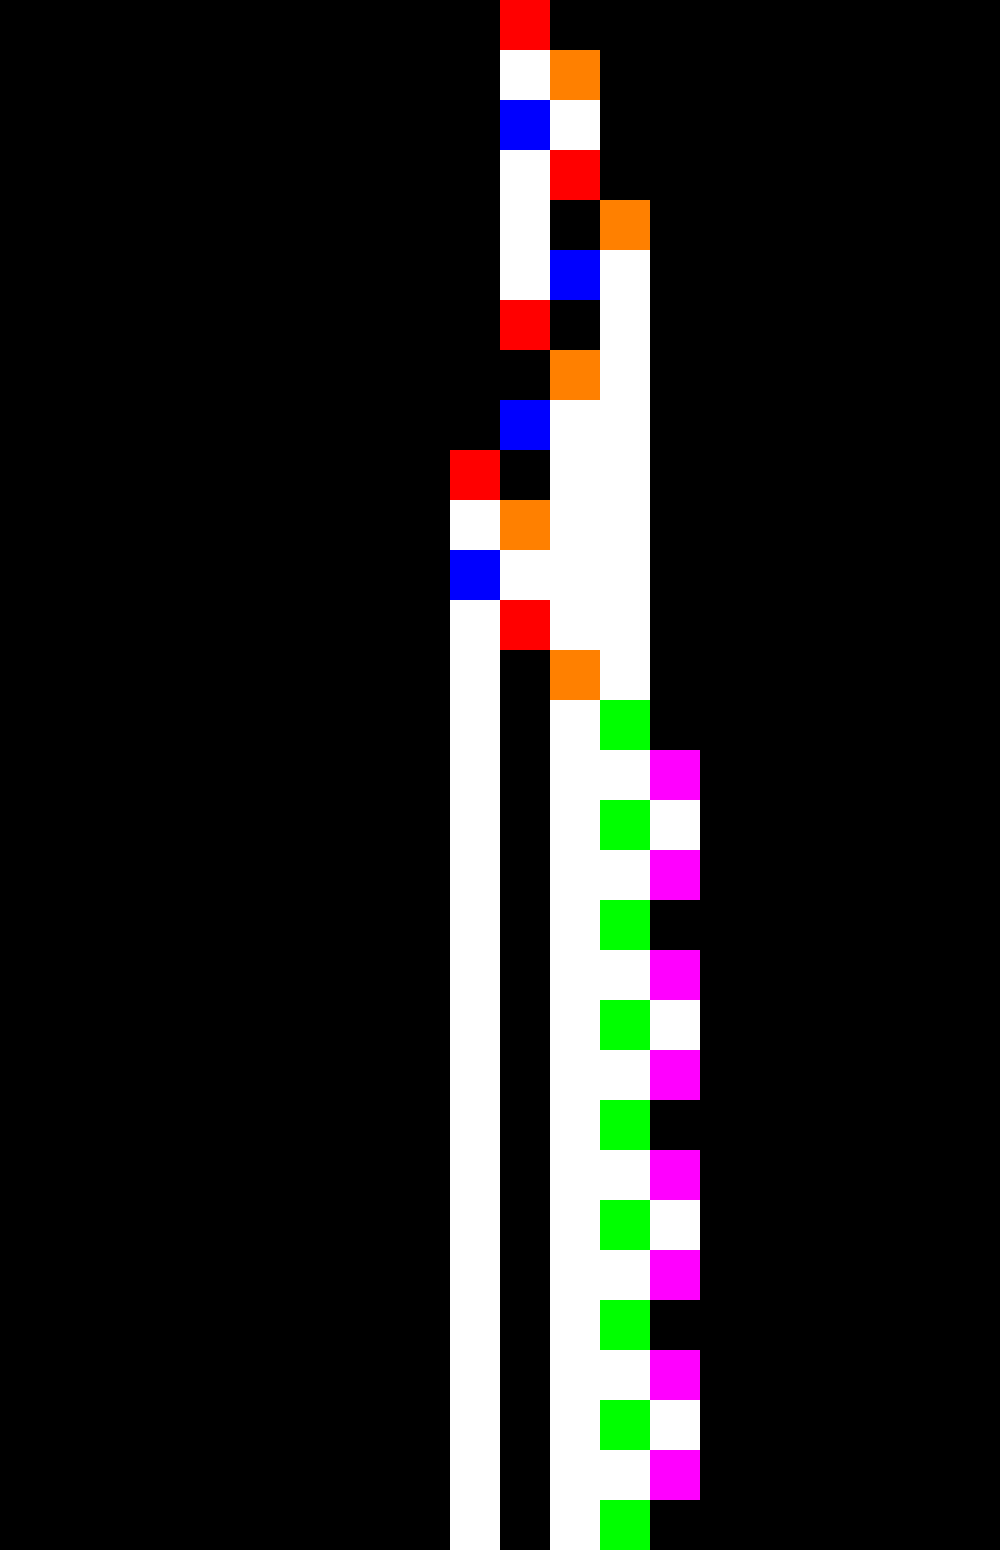
\includegraphics[width=0.4\textwidth]{figures/space-time-diagrams/cycler_4239083.pdf}
  \caption{Space-time diagrams of the 30 first steps of bbchallenge's machines \#279,081 (left) and \#4,239,083 (right) which are both ``Cyclers'': they eventually repeat the same configuration for ever. \\
    Access the machines at \url{https://bbchallenge.org/279081} and
    \url{https://bbchallenge.org/4239083}.}\label{fig:cyclers}
\end{figure}

The goal of this decider is to recognise Turing machines that cycle through the same configurations forever. Such machines never halt. The method is simple: remember every configuration seen by a machine and return \texttt{true} if one is visited twice. A time limit (maximum number of steps) is also given for running the test in practice: the algorithm recognises any machine whose cycle fits within this limit\footnote{In practice, for machines with 5 states the decider was run with 1000 steps time limit.}.


\begin{example}\normalfont
  Figure~\ref{fig:cyclers} gives the space-time diagrams of the 30 first iterations of two ``Cyclers'' machines: bbchallenge's machines \#279,081 (left) and \#4,239,083 (right). Refer to \url{https://bbchallenge.org/279081} and
  \url{https://bbchallenge.org/4239083} for their transition tables. From these space-time diagrams we see that the machines eventually repeat the same configuration.
\end{example}

\subsection{Pseudocode}

We assume that we are given a Turing Machine type \textbf{TM} that encodes the transition table of a machine as well as a procedure \textbf{TuringMachineStep}(machine,configuration) which computes the next configuration of a Turing machine from the given configuration or \textbf{nil} if the machine halts at that step. The pseudocode is given in Algorithm~\ref{alg:cyclers}.

\begin{algorithm}
  \caption{{\sc decider-cyclers}}\label{alg:cyclers}

  \begin{algorithmic}[1]

    \State \textbf{struct} Configuration \{
    \State \tabi\textbf{State} state
    \State \tabi\textbf{int} headPosition
    \State \tabi\textbf{int $\boldsymbol{\to}$ int} tape
    \State \}
    \State
    \Procedure{\textbf{bool} {\sc decider-cyclers}}{\textbf{TM} machine,\textbf{int} timeLimit}
    \State \textbf{Configuration} currConfiguration = \{.state = \textcolor{colorA}{A}, .headPosition = 0, .tape = \{0:0\}\}
    \State \textbf{Set$\boldsymbol{<}$Configuration$\boldsymbol{>}$} configurationsSeen = \{\}
    \State \textbf{int} currTime = 0

    \While{currTime $\leq$ timeLimit}
    \If{currConfiguration \textbf{in} configurationsSeen} \label{j:alg:cyclers}
    \State \textbf{return} true
    \EndIf
    \State configurationsSeen.\textbf{insert}(currConfiguration) \label{i:alg:cyclers}

    \State currConfiguration = \textbf{TuringMachineStep}(machine,currConfiguration)
    \State currTime += 1


    \If{currConfiguration == \textbf{nil}}
    \State \textbf{return} false //machine has halted, it is not a Cycler
    \EndIf
    \EndWhile

    \State \textbf{return} false
    \EndProcedure

  \end{algorithmic}
\end{algorithm}

\subsection{Correctness}



\begin{theorem}\label{th:cyclers} Let $\mathcal{M}$ be a Turing machine and $t \in \mathbb{N}$ a time limit. Let $c_0$ be the initial configuration of the machine. There exists $i\in\mathbb{N}$ and $j\in\mathbb{N}$ such that $c_0 \vdash^i c_i \vdash^{j-i} c_i$ with $i < j \leq t$ if and only if {\sc decider-cyclers}($\mathcal{M}$,$t$) returns \texttt{true} (Algorithm~\ref{alg:cyclers}).
\end{theorem}
\begin{proof}
  This follows directly from the behavior of {\sc decider-cyclers}($\mathcal{M}$,$t$): all configurations from $c_0$ to $c_t$ are recorded and the algorithm returns \texttt{true} if and only if one is visited twice. This mathematically translates to
  there exists $i\in\mathbb{N}$ and $j\in\mathbb{N}$ such that $c_0 \vdash^i c_i \vdash^{j-i} c_i$ with $i < j \leq t$, which is what we want. Index $i$ corresponds to the first time that $c_i$ is seen (l.\ref{i:alg:cyclers} in Algorithm~\ref{alg:cyclers}) while index $j$ corresponds to the second time that $c_i$ is seen (l.\ref{j:alg:cyclers} in Algorithm~\ref{alg:cyclers}).
\end{proof}

\begin{corollary}
  Let $\mathcal{M}$ be a Turing machine and $t \in \mathbb{N}$ a time limit. If {\sc decider-cyclers}($\mathcal{M}$,$t$) returns \texttt{true} then the behavior of $\mathcal{M}$ from all-0 tape has been decided: $\mathcal{M}$ does not halt.
\end{corollary}
\begin{proof}
  By Theorem~\ref{th:cyclers}, there exists $i\in\mathbb{N}$ and $j\in\mathbb{N}$ such that $c_0 \vdash^i c_i \vdash^{j-i} c_i$ with $i < j \leq t$. It follows that for all $k\in\mathbb{N}$, $c_0 \vdash^{i+k(j-i)} c_i$. The machine never halts as it will visit $c_i$ infinitely often.
\end{proof}

\subsection{Results}

The decider was coded in \texttt{golang} and is accessible at this link: \url{https://github.com/bbchallenge/bbchallenge-deciders/tree/main/decider-cyclers}.

The decider found 11,229,238 ``Cyclers'', out of 88,664,064 machines in the seed database of the Busy Beaver Challenge (c.f. \url{https://bbchallenge.org/method#seed-database}). Time limit was set to 1000 and an additional memory limit (max number of visited cells) was set to 500. More information about these results are available at: \url{https://discuss.bbchallenge.org/t/decider-cyclers/33}.
